\documentclass[11pt]{article}
\usepackage[margin=1in]{geometry}
\usepackage{graphicx}
\usepackage[hidelinks]{hyperref}
\usepackage{parskip}
\setlength{\parskip}{0.65em}

\title{Homework 3: RLHF on CartPole}
\author{Fnu Mayank\\\texttt{mlnu@umass.edu}}
\date{CS 690S --- AI Alignment}

\begin{document}
\maketitle

\section*{Part 1: Synthetic demonstration generation}

I ran VPG on CartPole-v0 for 10 epochs with checkpoints saved under \texttt{synthetic/}. The policy was not trained to convergence since we only need suboptimal policies to generate preference data. Over 10 epochs, the mean episode return went from about 18 up to about 34, confirming the policy was improving but still far from the optimal return of 200.

\section*{Part 2: Pairwise preferences and reward function}

I implemented the reward network in \texttt{utils.py} as a 2-hidden-layer feedforward network (4 $\rightarrow$ 32 $\rightarrow$ 32 $\rightarrow$ 1) with ReLU activations. It takes a state and outputs a scalar reward; the cumulative return for a trajectory is the sum of per-step rewards.

In \texttt{offline\_reward\_learning.py}, I implemented \texttt{learn\_reward} using \texttt{CrossEntropyLoss} where the two logits are the predicted cumulative returns for each trajectory in a pair, and the label is 0 if the first trajectory has higher true return and 1 otherwise. The reward network was trained for 100 iterations over 20 pairwise preferences sampled from rollouts of the 10 synthetic checkpoints.

After training, all 20 preference pairs in the training set were ranked correctly by the learned reward: whenever the label said trajectory A should be preferred, the predicted return for A was higher than for B, and vice versa. The learned weights were saved as \texttt{reward.params}.

\section*{Part 3: RL on the learned reward function}

\subsection*{Training}

I ran VPG for 50 epochs using the learned reward function in place of the true CartPole reward, saving checkpoints under \texttt{rlhf/}. During training, the ground-truth episode length (which VPG logs but does not optimize directly) climbed steadily, reaching 200.0 at epoch 48 and staying near 200 through epoch 49. This confirms the learned reward aligns well with the true objective.

\subsection*{Evaluation}

CartPole's true return is $+1$ per step up to a maximum of 200. All evaluations below use the true environment reward (not the learned reward), with 5 rollouts each as the README specifies.

\begin{itemize}
  \setlength{\itemsep}{0.4em}
  \item \textbf{RLHF policy} (checkpoint 49): returns of 200, 200, 200, 200, and 200. Average: \textbf{200.0}.
  \item \textbf{Synthetic policy} (checkpoint 9): returns of 17, 18, 29, 45, and 21. Average: \textbf{26.0}.
\end{itemize}

\subsection*{Learning curve}

Figure~\ref{fig:curve} plots the mean ground-truth return (5 rollouts) at each of the 50 RLHF checkpoints. The curve starts around 20 and climbs steadily, first reaching 200.0 at checkpoint 39. Checkpoints 42--49 all averaged 200.0, showing the policy converged to near-optimal performance and stayed there.

\begin{figure}[htbp]
  \centering
  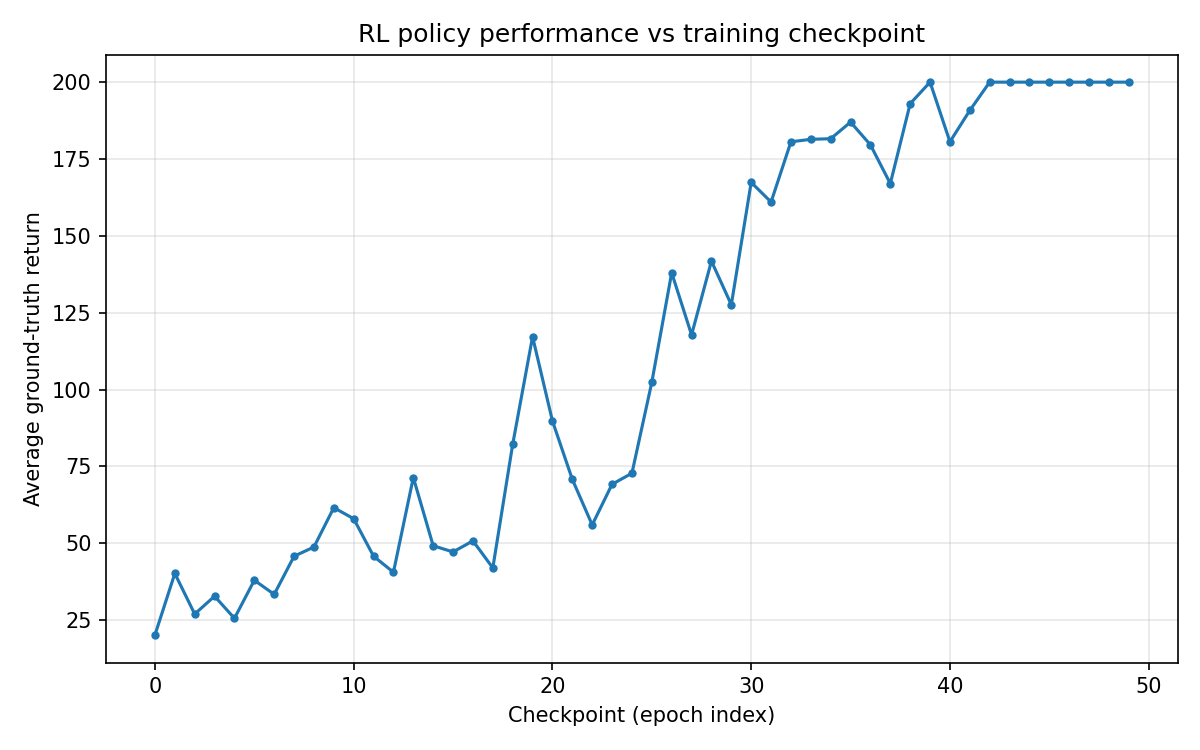
\includegraphics[width=0.85\textwidth]{rlhf_checkpoints.png}
  \caption{Mean CartPole return vs.\ RLHF checkpoint (5 rollouts per checkpoint).}
  \label{fig:curve}
\end{figure}

\subsection*{Questions}

\subsubsection*{(1) Was your RLHF method able to learn a better policy than the best policy used to collect training data?}

Yes. The preference dataset came from rollouts of ten synthetic policies (checkpoints 0--9). The best single trajectory return among those rollouts was 64, and evaluating the final synthetic checkpoint by itself gave an average of only 26.0. The RLHF policy averaged 200.0 over five rollouts, all hitting the maximum. So RLHF clearly produced a much better policy than anything used to generate the preference data.

\subsubsection*{(2) Why is it possible to learn a policy much better than the best trajectory in the training data?}

We never trained the policy to imitate a trajectory. We trained a reward model from pairwise preferences: for two trajectories, which one has higher true return? The logits in the cross-entropy loss were the predicted cumulative returns, and the label was which trajectory should be preferred. This gives the reward function a notion of what ``better'' looks like without capping it at the quality of any single demo.

Once we have a reward function that correlates with keeping the pole up longer, RL can keep exploring in the real environment and find behavior that was never in the offline data, including episodes that last all 200 steps. The best offline trajectory was 64 steps, but RL is not limited to replaying logged trajectories; it optimizes new ones under the learned reward.

\subsubsection*{(3) Explain how RLHF is different from Inverse RL or behavioral cloning.}

\textbf{Behavioral cloning (BC)} is supervised learning on state-action pairs from demonstrations. The policy learns to predict what action was taken, not what action leads to high return. If demos are suboptimal, BC inherits that. It also suffers from compounding error when the learned policy drifts from the demo distribution.

\textbf{Inverse RL (IRL)} assumes demonstrations from an approximately optimal policy and tries to recover a reward function that makes those demonstrations look near-optimal. It then derives a policy from that reward. The setup is different: it needs expert-quality data and often uses specific constraints to resolve reward ambiguity.

\textbf{What we did (RLHF)} learns a reward from pairwise trajectory preferences using a classification loss, then runs policy gradient on the learned reward. The supervision signal is relative rankings (``this trajectory is better than that one''), not expert actions or an assumption of optimality. This lets us extract useful reward information even from suboptimal data.

\subsubsection*{(4) What would have happened if you ran Inverse RL or behavioral cloning on the same trajectories used for RLHF?}

\textbf{BC} would try to copy the state-action mappings from those weak policies. Since the demos only averaged around 20--60 return, BC would likely produce a policy in that same range or worse due to compounding error. BC does not use the preference labels, so it throws away the signal that one trajectory is better than another.

\textbf{IRL} would try to find a reward that explains the observed behavior as if it were optimal. With only suboptimal demonstrations, IRL could fit a reward that rationalizes mediocre behavior, which would not push a policy toward CartPole's true objective. IRL also does not use pairwise preference labels; it works from trajectories alone under different assumptions.

Neither method would replicate the RLHF result because they do not use the pairwise comparison signal, and they are not designed to extrapolate beyond the quality of the demonstrations.

\end{document}
